% This is samplepaper.tex, a sample chapter demonstrating the
% LLNCS macro package for Springer Computer Science proceedings;
% Version 2.21 of 2022/01/12
%
\documentclass[runningheads]{llncs}
%
\usepackage[T1]{fontenc}
% T1 fonts will be used to generate the final print and online PDFs,
% so please use T1 fonts in your manuscript whenever possible.
% Other font encondings may result in incorrect characters.
%
\usepackage{graphicx}
\usepackage{subcaption}
% Used for displaying a sample figure. If possible, figure files should
% be included in EPS format.
%
% If you use the hyperref package, please uncomment the following two lines
% to display URLs in blue roman font according to Springer's eBook style:
%\usepackage{color}
%\renewcommand\UrlFont{\color{blue}\rmfamily}
%\urlstyle{rm}
%
\begin{document}
%
\title{Neonatal Brain MRI Segmentation}
%
%\titlerunning{Abbreviated paper title}
% If the paper title is too long for the running head, you can set
% an abbreviated paper title here
%
\author{Ľubomír Hlavko  %\orcidID0000-1111-2222-3333}
\and
Jan Platoš %\orcidID{1111-2222-3333-4444} 
\and
Dominik Vilímek %\orcidID{2222--3333-4444-5555}}
%
%\authorrunning{F. Author et al.
}
% First names are abbreviated in the running head.
% If there are more than two authors, 'et al.' is used.
%
\institute{VSB - Technical University of Ostrava 17. listopadu 2172/15, 708 00 Ostrava-Poruba, Czech Republic %\and
%Springer Heidelberg, Tiergartenstr. 17, 69121 Heidelberg, Germany
%\email{lncs@springer.com}\\
%\url{http://www.springer.com/gp/computer-science/lncs} \and
%ABC Institute, Rupert-Karls-University Heidelberg, Heidelberg, Germany\\
%\email{\{abc,lncs\}@uni-heidelberg.de}
}
%
\maketitle              % typeset the header of the contribution
%
\begin{abstract}
The study focuses on semantic segmentation of neonatal brain images obtained by magnetic resonance imaging. Deep neural networks for semantic segmentation were selected, implemented, or existing implementations were utilized. The networks were used on available datasets from the iSeg 2019 and BONBID-HIE 2023 challenges and also our internal dataset TAČR 6-HIE to perform 4 segmentation tasks in total. The networks were evaluated using selected metrics and are presented in this study. 

\keywords{Neonatal MRI \and Semantic segmentation \and Computer Vision \and Medical image analysis \and Hypoxic Ischemic Encephalopathy \and HIE.}
\end{abstract}

\section{Introduction}
Magnetic resonance imaging is a noninvasive technique for examining tissues in (living) organisms. The examination is recommended for newborns with neurological disorders, suspected brain damage, injuries, or malformations (e.g., hypoxic-ischemic encephalopathy), seizures, or head trauma \cite{csnn,neonatal_technical,bonbid}. Images can be used to detect and examine extend and location of brain abnormalities and accurate segmentation might be helpful. The imaging and segmentation is more challenging than in adults due to lower resolution, low contrast, and unclear tissue contrast distribution. Around 6 months of age, MRI voxel intensities of white and gray matter overlap significantly, making the segmentation even harder. As a result, segmentation tools developed for adults often perform poorly on infant brain images \cite{iseg2019}. As a result specialized tools have been (or are actively) developed and deep neural networks for semantic segmenations can be utilized.

%\section{Related work}
%Neonatal brain MRI segmentation is an active area of research. Challenges which focus on this topic were also held such as the Iseg 2019 \cite{iseg2019} and  BONBID-HIE 2023 \cite{bonbid} challenge. Many architectures and models were proposed for these specific challenges. Semantic segmentation of medical images in general is also an active area of research with . Specialized or general solutions are being developed. 

\section{Datasets}
Datasets from mentioned challenges were utilized and also internal dataset TAČR 6 - HIE which is being gathered in collaboration with Faculty hospital of Ostrava. Usage of the anonymized data in this study is compliant with the ethics. 

ISeg 2019 contains processed images of infants aged around 6 months and the segmentation is classifiing voxels as white matter, dark matter and cerebrospinal fluid. We use subjects for which two images and ground truth mask is available. More details for the dataset can be found out in article \cite{iseg2019}. 

BONBID-HIE 2023 dataset \cite{bonbid} contains images of infants diagnosed with hypoxic-ischemic encephalopathy (HIE), and the task is to segment whether the voxel contains tissue damaged by HIE or not. The images have different sizes and voxel sizes and for processing the images are resampled to unified size of 256 x 256 x 64 with 1mm x1 mm x1 mm voxel size. 2 images and one ground truth mask per subject is available. The amount of the brain tissue affected is different across the images.

The TAČR 6 - HIE dataset contains images of 1 to 2 day old newborns diagnosed with HIE. The images were captured by Siemens Prisma 3 tesla magnetic resonance using 32 channel head coil. The images were preprocessed using N4 bias correction, skull striping and anonymized. After that, ground truth anatomical segmentation maps created using FreeSurfer infant pipeline \cite{freesurfer_infant} were created. Images for 20 subjects were provided for writing of this study.

\begin{table}
\caption{Overview of datasets}
\label{tab:datasetsSummary}
\centering
\begin{tabular}{p{3cm} c c c}
\hline
Parameter & iSeg 2019 & BONBID-HIE 2023 & TAČR 6 - HIE \\
\hline
Number of subjects & 10 & 81 & 20 \\
Images per subject & 2 & 2 & 1 \\
Image size & 256 x 160 x 144 & various & 256 x 256 x 256\\
Number of classes  & 4 & 2 & 31, 98 \\
\hline
\end{tabular}
\end{table}

All the datasets have imbalanced classess, background is most prelevant class in all of them, but also the number of voxels representing brain tissue classes is imbalanced. Class imbalance is typical for medical image analysis and should be taken into account \cite{loss_odyssey}. Example slices of images for datasets are in figure \ref{fig:datasetsExamples}.

\begin{figure}[h]
    \centering
        \begin{subfigure}{\textwidth}
   \centering
            
\includegraphics[width=0.2\textwidth]{Data/iseg2019_dataset/slices/training/2_1.png}
            
\includegraphics[width=0.2\textwidth]{Data/iseg2019_dataset/slices/training/2_2.png}
            
\includegraphics[width=0.2\textwidth]{Data/iseg2019_dataset/slices/training/2_3.png}
            \caption{iSeg 2019 subject (T1, T2 and segmentation map)}
        \end{subfigure}
        \begin{subfigure}{\textwidth}
   \centering
            
\includegraphics[width=0.2\textwidth]{Data/bonbid2023_dataset/slices/training/3_1.png}
            
\includegraphics[width=0.2\textwidth]{Data/bonbid2023_dataset/slices/training/3_2.png}
            
\includegraphics[width=0.2\textwidth]{Data/bonbid2023_dataset/slices/training/3_3.png}
            \caption{BONBID-HIE 2023 subject (ADC, Z\_ADC and segmentation map)}
        \end{subfigure}
        \begin{subfigure}{\textwidth}
   \centering
            
\includegraphics[width=0.2\textwidth]{Data/tacrhie_dataset/slices/training/5_1.png}
            
\includegraphics[width=0.2\textwidth]{Data/tacrhie_dataset/slices/training/5_2.png}
            
\includegraphics[width=0.2\textwidth]{Data/tacrhie_dataset/slices/training/5_3.png}
            \caption{TAČR 6 - HIE subject (T1, aseg and aseg+aparc segmentation maps)}
        \end{subfigure}
    \hfill

\caption{Examples of datasets images.}
\label{fig:datasetsExamples}
\end{figure}

\section{Methodology}
\label{sec:methodology}
Same training, validation and testing images were used for training and evaluating every model. The datasets were split for training, testing and validation parts in ratio 80:10:10. Models were evaluated using metrics. We opted for metrics for binary segmentation, namely DICE coefficient,  Hausdorff distance, Mutual information, Mahalanobis distance and Volumetric similarity for evaluating models. DICE coefficient was chosen as it is one of the most used metric \cite{metrics_for_evaluating} for evaluating semantic segmentation. Hausdorff distance and Mahalanobis distances were chosen from distance based metrics. Volumetric similarity was chosen because it measures the similarity from the point of volumes of segmented segements. Mutual information was chosen because it quantifies the amount of shared information between the predicted segmentation and the ground truth, making it effective for evaluating alignment and overall structural similarity. Definitions of metrics and utilized tool were also described in mentioned article \cite{metrics_for_evaluating}. For multiclass segmentations such as in case of iSeg 2019 and TAČR 6 - HIE segmentation tasks, weighted average of inidividual classes metrics were calculated to get agregated results for whole images. Relative volumes of classes in ground truth segmentation masks were used as coresponding weights.

\section{Selected Models}
\label{sec:models}
We implemented convolutional neural networks based on architectures such as U-net \cite{unet} and DeepLab version 3 \cite{deeplab}. From existing implementations, we opted for nnUNet version 2, which is an automated tool developed for the semantic segmentation of medical images using the U-net architecture \cite{nnunet}. We compared both 2D and 3D full resolution configurations for all datasets. The seond tool used was U-mamba, which is based on nnUnet which utilizes sequence state space based architecture implementation called Mamba \cite{mamba}. Similarly 2D and 3D full resolution configurations,  which use Mamba block only within the network's bottlenek were used. Source codes are available in repository \cite{repository}.
 
\section{Results}
We trained, tested and evaluated models mentioned in section \ref{sec:models} using methodology specified in section \ref{sec:methodology}. Table \ref{tab:bonbidstats} contains medians and IQRs of metrics calculated for testing subjects of dataset BONBID-HIE 2023, table \ref{tab:isegstats} for iSeg 2019, tables \ref{tab:tacrasegstats} and \ref{tab:tacraparcstats} for TAČR 6 - HIE datasets. Images \ref{fig:isegslicecomparison}, \ref{fig:bonbidslicecomparison}, \ref{fig:tacrasegslicecomparison} and \ref{fig:tacrasegslicecomparison} show visual comparison of one slice of resulting segmentations for testing subjects of respective datasets and ground truth. Incorrectly segmented voxels have got dark red colour. Next list briefly describes the results for each segmentation task.

\begin{itemize}
\item According to the results in table \ref{tab:bonbidstats}, the nnUNet (3D) model achieved the highest median DICE similarity in the BONBID-HIE 2023 test dataset. The 2D configuration reached a higher MI value with a smaller interquartile range. The custom implementation of the DeepLab v3 model achieved a lower median DICE similarity with a larger interquartile range. The smallest Hausdorff distance was obtained by the U-Mamba model with the 3D bottleneck configuration, while DeepLab v3 showed a higher median with smaller IQR. The highest volume similarity and Mahalanobis distance were reached by the DeepLab v3 model.

\item According to the table \ref{tab:isegstats}, the nnUNet (3D) model achieved the highest DICE similarity and MI on the iSeg 2019 test dataset. The 2D configuration of nnUNet achieved the smallest Mahalanobis distance. The highest volume similarity was reached by the U-Mamba model 2D bottleneck configuration. The smallest Hausdorff distance was achieved by the 3D bottleneck configuration. 

\item According to the results in table \ref{tab:tacrasegstats}, the custom implementation of U-Net (3D) achieved the highest median DICE similarity, the lowest median Hausdorff distance, the highest MI value, and the lowest median MHD on the TAČR 6-HIE (aseg) test dataset. Only the U-Mamba 3D bottleneck configuration reached a higher volume similarity. 

\item According to the results in table \ref{tab:tacraparcstats}, the custom implementation of U-Net (3D) also achieved the highest median DICE similarity, the highest MI value, and the lowest median MHD in the TAČR 6-HIE (aseg+aparc) test dataset. The nnUNet in the 3D configuration achieved a lower Hausdorff distance but with a larger interquartile range. Only the U-Mamba model in the 3D bottleneck configuration achieved a higher volume similarity.
\end{itemize}

\begin{table}
\centering
\caption{Medians and IQR of achieved metrics in BONBID-HIE 2023 segmentation. Maximal medians of similarities and mutual information and minimal medians of distances are highlighted.}
\label{tab:bonbidstats}
\scriptsize
\begin{tabular}{l c c c c c}
 \hline
Model & DICE & HD & VS & MI & MHD \\ \hline
U-net (3D) & 0,000 (0,015) & 162,123 (43,861) & 0,017 (0,325) & 0,000 (0,000) & 5,858 (66,481) \\ 
nnUnet (2D) & 0,087 (0,363) & 49,123 (36,847) & 0,213 (0,504) & \textbf{0,002 (0,010)} & 0,953 (0,617) \\ 
nnUnet (3D) & \textbf{0,408 (0,190)} & 32,997 (16,728) & 0,671 (0,418) & 0,002 (0,011) & 0,631 (0,841) \\ 
DeepLab (v3) & 0,407 (0,299) & 31,443 (14,896) & \textbf{0,740 (0,125)} & 0,001 (0,008) & \textbf{0,481 (0,444)} \\ 
U-Mamba (2D bot) & 0,064 (0,407) & 51,862 (41,881) & 0,190 (0,780) & 0,002 (0,010) & 0,915 (0,665) \\ 
U-Mamba (3D bot) & 0,168 (0,343) & \textbf{30,564 (22,293)} & 0,586 (0,254) & 0,001 (0,011) & 0,941 (0,831) \\ 
\hline 
 \end{tabular}

\end{table}

\begin{table}
\centering
\caption{Medians and IQR of achieved metrics in iSeg 2019 segmentation. Maximal medians of similarities and mutual information and minimal medians of distances are highlighted.}
\label{tab:isegstats}
\scriptsize
\input{Data/results/iseg2019_stats.tex}
\end{table}

\begin{table}
\centering
\caption{Medians and IQR of achieved metrics in TAČR 6 - HIE aseg segmentation. Maximal medians of similarities and mutual information and minimal medians of distances are highlighted.}
\label{tab:tacrasegstats}
\scriptsize
\begin{tabular}{l c c c c c}
 \hline
Model & DICE & HD & VS & MI & MHD \\ \hline
U-net (3D) & \textbf{0,751 (0,012)} & \textbf{20,546 (2,143)} & 0,929 (0,013) & \textbf{0,021 (0,001)} & \textbf{0,200 (0,054)} \\ 
nnUnet (2D) & 0,635 (0,083) & 40,181 (0,383) & 0,980 (0,003) & 0,015 (0,003) & 0,733 (0,230) \\ 
nnUnet (3D) & 0,463 (0,438) & 23,678 (18,092) & 0,983 (0,004) & 0,013 (0,013) & 1,999 (1,953) \\ 
DeepLab (v3) & 0,066 (0,022) & 63,642 (1,331) & 0,766 (0,169) & 0,001 (0,000) & 4,266 (0,285) \\ 
U-Mamba (2D bot) & 0,673 (0,086) & 40,393 (0,570) & 0,981 (0,005) & 0,017 (0,003) & 0,616 (0,258) \\ 
U-Mamba (3D bot) & 0,459 (0,434) & 23,832 (17,829) & \textbf{0,985 (0,005)} & 0,013 (0,013) & 1,998 (1,947) \\ 
\hline 
 \end{tabular}

\end{table}

\begin{table}
\centering
\caption{Medians and IQR of achieved metrics in TAČR 6 - HIE aseg+aparc segmentation. Maximal medians of similarities and mutual information and minimal medians of distances are highlighted.}
\label{tab:tacraparcstats}
\scriptsize
\begin{tabular}{l c c c c c}
 \hline
Model & DICE & HD & VS & MI & MHD \\ \hline
U-net (3D) & \textbf{0,645 (0,010)} & 24,705 (2,323) & 0,872 (0,006) & \textbf{0,014 (0,000)} & \textbf{0,448 (0,066)} \\ 
nnUnet (2D) & 0,577 (0,116) & 34,658 (2,075) & 0,948 (0,012) & 0,009 (0,003) & 0,885 (0,418) \\ 
nnUnet (3D) & 0,423 (0,399) & \textbf{21,813 (16,192)} & 0,957 (0,010) & 0,007 (0,007) & 3,060 (2,896) \\ 
DeepLab (v3) & 0,045 (0,007) & 66,577 (3,306) & 0,646 (0,186) & 0,001 (0,000) & 6,997 (0,785) \\ 
U-Mamba (2D bot) & 0,150 (0,011) & 29,035 (0,894) & 0,316 (0,012) & 0,004 (0,001) & 1,718 (0,151) \\ 
U-Mamba (3D bot) & 0,416 (0,392) & 21,858 (16,168) & \textbf{0,957 (0,009)} & 0,007 (0,007) & 3,053 (2,880) \\ 
\hline 
 \end{tabular}

\end{table}


%\begin{figure}
%\centering
%\input{original_bonbid_eng.tex}
%\end{figure}

%\begin{figure}
%\centering
%\input{resized_bonbid_eng.tex}
%\end{figure}

\begin{figure}
\centering
\begin{minipage}{\textwidth}
\centering
\begin{minipage}{0.33\textwidth}
\hfill
\begin{minipage}{0.3\textwidth}
\rotatebox{90}{1. Image}
\end{minipage}
\hfill
\begin{minipage}{0.3\textwidth}
\rotatebox{90}{2. Image}
\end{minipage}
\hfill
\begin{minipage}{0.3\textwidth}
\rotatebox{90}{Ground truth}
\end{minipage}
\hfill
\end{minipage}
\begin{minipage}{0.099\textwidth}
\centering
\rotatebox{90}{U-net (3D)}
\end{minipage}
\begin{minipage}{0.099\textwidth}
\centering
\rotatebox{90}{nnUNet (2D)}
\end{minipage}
\begin{minipage}{0.099\textwidth}
\centering
\rotatebox{90}{nnUNet (3D)}
\end{minipage}
\begin{minipage}{0.099\textwidth}
\centering
\rotatebox{90}{DeepLab (v3)}
\end{minipage}
\begin{minipage}{0.099\textwidth}
\centering
\rotatebox{90}{U-Mamba (2D bot)}
\end{minipage}
\begin{minipage}{0.099\textwidth}
\centering
\rotatebox{90}{U-Mamba (3D bot)}
\end{minipage}
\end{minipage}
\begin{minipage}{\textwidth}
\centering
\begin{minipage}{0.33\textwidth}
\centering
\rotatebox{90}{\tiny \textbf{Subject 1} }

\includegraphics[width=0.3\textwidth]{Data/results//Unet/iSeg 2019/1_1.nii_src_2.png}%

\includegraphics[width=0.3\textwidth]{Data/results//Unet/iSeg 2019/1_1.nii_src2_2.png}%

\includegraphics[width=0.3\textwidth]{Data/results//Unet/iSeg 2019/1_1.nii_gt_2.png}
\end{minipage}
\begin{minipage}{0.099\textwidth}
\centering

\includegraphics[width=\textwidth]{Data/results//Unet/iSeg 2019/1_1.nii_seg_err_2.png}
\end{minipage}
\begin{minipage}{0.099\textwidth}
\centering

\includegraphics[width=\textwidth]{Data/results//nnUNet2_2d/iSeg 2019/1_1.nii_seg_err_2.png}
\end{minipage}
\begin{minipage}{0.099\textwidth}
\centering

\includegraphics[width=\textwidth]{Data/results//nnUNet2_3d_fullres/iSeg 2019/1_1.nii_seg_err_2.png}
\end{minipage}
\begin{minipage}{0.099\textwidth}
\centering

\includegraphics[width=\textwidth]{Data/results//Deeplabv3/iSeg 2019/1_1.nii_seg_err_2.png}
\end{minipage}
\begin{minipage}{0.099\textwidth}
\centering

\includegraphics[width=\textwidth]{Data/results//UMamba_2d_bot/iSeg 2019/1_1.nii_seg_err_2.png}
\end{minipage}
\begin{minipage}{0.099\textwidth}
\centering

\includegraphics[width=\textwidth]{Data/results//UMamba_3d_bot/iSeg 2019/1_1.nii_seg_err_2.png}
\end{minipage}
\end{minipage}\\%

\vspace{0.05cm}

\caption{Visual comparison of slices of images, ground truth and segmentations created by models for iSeg2019 segmentations. Incorrectly classified pixels are dark red.}
\label{fig:isegslicecomparison}
\end{figure}

\begin{figure}
\centering
\begin{minipage}{\textwidth}
\centering
\begin{minipage}{0.33\textwidth}
\hfill
\begin{minipage}{0.3\textwidth}
\rotatebox{90}{1. Image}
\end{minipage}
\hfill
\begin{minipage}{0.3\textwidth}
\rotatebox{90}{2. Image}
\end{minipage}
\hfill
\begin{minipage}{0.3\textwidth}
\rotatebox{90}{Ground truth}
\end{minipage}
\hfill
\end{minipage}
\begin{minipage}{0.099\textwidth}
\centering
\rotatebox{90}{U-net (3D)}
\end{minipage}
\begin{minipage}{0.099\textwidth}
\centering
\rotatebox{90}{nnUNet (2D)}
\end{minipage}
\begin{minipage}{0.099\textwidth}
\centering
\rotatebox{90}{nnUNet (3D)}
\end{minipage}
\begin{minipage}{0.099\textwidth}
\centering
\rotatebox{90}{DeepLab (v3)}
\end{minipage}
\begin{minipage}{0.099\textwidth}
\centering
\rotatebox{90}{U-Mamba (2D bot)}
\end{minipage}
\begin{minipage}{0.099\textwidth}
\centering
\rotatebox{90}{U-Mamba (3D bot)}
\end{minipage}
\end{minipage}
\begin{minipage}{\textwidth}
\centering
\begin{minipage}{0.33\textwidth}
\centering
\rotatebox{90}{\tiny \textbf{Subject 1} }
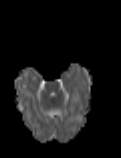
\includegraphics[width=0.3\textwidth]{Data/results//Unet/BONBID-HIE 2023/1_1.nii_src_2.png}%
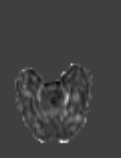
\includegraphics[width=0.3\textwidth]{Data/results//Unet/BONBID-HIE 2023/1_1.nii_src2_2.png}%

\includegraphics[width=0.3\textwidth]{Data/results//Unet/BONBID-HIE 2023/1_1.nii_gt_2.png}
\end{minipage}
\begin{minipage}{0.099\textwidth}
\centering

\includegraphics[width=\textwidth]{Data/results//Unet/BONBID-HIE 2023/1_1.nii_seg_err_2.png}
\end{minipage}
\begin{minipage}{0.099\textwidth}
\centering

\includegraphics[width=\textwidth]{Data/results//nnUNet2_2d/BONBID-HIE 2023/1_1.nii_seg_err_2.png}
\end{minipage}
\begin{minipage}{0.099\textwidth}
\centering

\includegraphics[width=\textwidth]{Data/results//nnUNet2_3d_fullres/BONBID-HIE 2023/1_1.nii_seg_err_2.png}
\end{minipage}
\begin{minipage}{0.099\textwidth}
\centering

\includegraphics[width=\textwidth]{Data/results//Deeplabv3/BONBID-HIE 2023/1_1.nii_seg_err_2.png}
\end{minipage}
\begin{minipage}{0.099\textwidth}
\centering

\includegraphics[width=\textwidth]{Data/results//UMamba_2d_bot/BONBID-HIE 2023/1_1.nii_seg_err_2.png}
\end{minipage}
\begin{minipage}{0.099\textwidth}
\centering

\includegraphics[width=\textwidth]{Data/results//UMamba_3d_bot/BONBID-HIE 2023/1_1.nii_seg_err_2.png}
\end{minipage}
\end{minipage}\\%

\vspace{0.05cm}
\begin{minipage}{\textwidth}
\centering
\begin{minipage}{0.33\textwidth}
\centering
\rotatebox{90}{\tiny \textbf{Subject 2} }
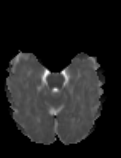
\includegraphics[width=0.3\textwidth]{Data/results//Unet/BONBID-HIE 2023/2_1.nii_src_2.png}%
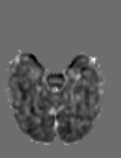
\includegraphics[width=0.3\textwidth]{Data/results//Unet/BONBID-HIE 2023/2_1.nii_src2_2.png}%
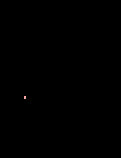
\includegraphics[width=0.3\textwidth]{Data/results//Unet/BONBID-HIE 2023/2_1.nii_gt_2.png}
\end{minipage}
\begin{minipage}{0.099\textwidth}
\centering

\includegraphics[width=\textwidth]{Data/results//Unet/BONBID-HIE 2023/2_1.nii_seg_err_2.png}
\end{minipage}
\begin{minipage}{0.099\textwidth}
\centering

\includegraphics[width=\textwidth]{Data/results//nnUNet2_2d/BONBID-HIE 2023/2_1.nii_seg_err_2.png}
\end{minipage}
\begin{minipage}{0.099\textwidth}
\centering

\includegraphics[width=\textwidth]{Data/results//nnUNet2_3d_fullres/BONBID-HIE 2023/2_1.nii_seg_err_2.png}
\end{minipage}
\begin{minipage}{0.099\textwidth}
\centering
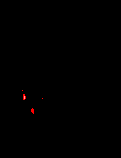
\includegraphics[width=\textwidth]{Data/results//Deeplabv3/BONBID-HIE 2023/2_1.nii_seg_err_2.png}
\end{minipage}
\begin{minipage}{0.099\textwidth}
\centering

\includegraphics[width=\textwidth]{Data/results//UMamba_2d_bot/BONBID-HIE 2023/2_1.nii_seg_err_2.png}
\end{minipage}
\begin{minipage}{0.099\textwidth}
\centering

\includegraphics[width=\textwidth]{Data/results//UMamba_3d_bot/BONBID-HIE 2023/2_1.nii_seg_err_2.png}
\end{minipage}
\end{minipage}\\%

\vspace{0.05cm}
\begin{minipage}{\textwidth}
\centering
\begin{minipage}{0.33\textwidth}
\centering
\rotatebox{90}{\tiny \textbf{Subject 3} }
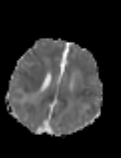
\includegraphics[width=0.3\textwidth]{Data/results//Unet/BONBID-HIE 2023/3_1.nii_src_2.png}%
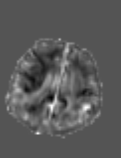
\includegraphics[width=0.3\textwidth]{Data/results//Unet/BONBID-HIE 2023/3_1.nii_src2_2.png}%
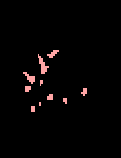
\includegraphics[width=0.3\textwidth]{Data/results//Unet/BONBID-HIE 2023/3_1.nii_gt_2.png}
\end{minipage}
\begin{minipage}{0.099\textwidth}
\centering

\includegraphics[width=\textwidth]{Data/results//Unet/BONBID-HIE 2023/3_1.nii_seg_err_2.png}
\end{minipage}
\begin{minipage}{0.099\textwidth}
\centering

\includegraphics[width=\textwidth]{Data/results//nnUNet2_2d/BONBID-HIE 2023/3_1.nii_seg_err_2.png}
\end{minipage}
\begin{minipage}{0.099\textwidth}
\centering

\includegraphics[width=\textwidth]{Data/results//nnUNet2_3d_fullres/BONBID-HIE 2023/3_1.nii_seg_err_2.png}
\end{minipage}
\begin{minipage}{0.099\textwidth}
\centering
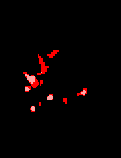
\includegraphics[width=\textwidth]{Data/results//Deeplabv3/BONBID-HIE 2023/3_1.nii_seg_err_2.png}
\end{minipage}
\begin{minipage}{0.099\textwidth}
\centering

\includegraphics[width=\textwidth]{Data/results//UMamba_2d_bot/BONBID-HIE 2023/3_1.nii_seg_err_2.png}
\end{minipage}
\begin{minipage}{0.099\textwidth}
\centering

\includegraphics[width=\textwidth]{Data/results//UMamba_3d_bot/BONBID-HIE 2023/3_1.nii_seg_err_2.png}
\end{minipage}
\end{minipage}\\%

\vspace{0.05cm}
\begin{minipage}{\textwidth}
\centering
\begin{minipage}{0.33\textwidth}
\centering
\rotatebox{90}{\tiny \textbf{Subject 4} }
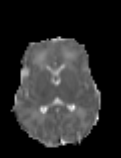
\includegraphics[width=0.3\textwidth]{Data/results//Unet/BONBID-HIE 2023/4_1.nii_src_2.png}%
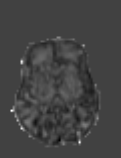
\includegraphics[width=0.3\textwidth]{Data/results//Unet/BONBID-HIE 2023/4_1.nii_src2_2.png}%

\includegraphics[width=0.3\textwidth]{Data/results//Unet/BONBID-HIE 2023/4_1.nii_gt_2.png}
\end{minipage}
\begin{minipage}{0.099\textwidth}
\centering

\includegraphics[width=\textwidth]{Data/results//Unet/BONBID-HIE 2023/4_1.nii_seg_err_2.png}
\end{minipage}
\begin{minipage}{0.099\textwidth}
\centering

\includegraphics[width=\textwidth]{Data/results//nnUNet2_2d/BONBID-HIE 2023/4_1.nii_seg_err_2.png}
\end{minipage}
\begin{minipage}{0.099\textwidth}
\centering

\includegraphics[width=\textwidth]{Data/results//nnUNet2_3d_fullres/BONBID-HIE 2023/4_1.nii_seg_err_2.png}
\end{minipage}
\begin{minipage}{0.099\textwidth}
\centering

\includegraphics[width=\textwidth]{Data/results//Deeplabv3/BONBID-HIE 2023/4_1.nii_seg_err_2.png}
\end{minipage}
\begin{minipage}{0.099\textwidth}
\centering

\includegraphics[width=\textwidth]{Data/results//UMamba_2d_bot/BONBID-HIE 2023/4_1.nii_seg_err_2.png}
\end{minipage}
\begin{minipage}{0.099\textwidth}
\centering

\includegraphics[width=\textwidth]{Data/results//UMamba_3d_bot/BONBID-HIE 2023/4_1.nii_seg_err_2.png}
\end{minipage}
\end{minipage}\\%

\vspace{0.05cm}
\begin{minipage}{\textwidth}
\centering
\begin{minipage}{0.33\textwidth}
\centering
\rotatebox{90}{\tiny \textbf{Subject 5} }
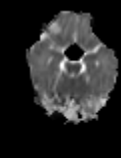
\includegraphics[width=0.3\textwidth]{Data/results//Unet/BONBID-HIE 2023/5_1.nii_src_2.png}%
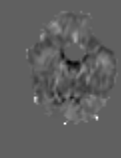
\includegraphics[width=0.3\textwidth]{Data/results//Unet/BONBID-HIE 2023/5_1.nii_src2_2.png}%
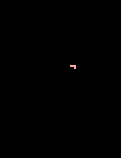
\includegraphics[width=0.3\textwidth]{Data/results//Unet/BONBID-HIE 2023/5_1.nii_gt_2.png}
\end{minipage}
\begin{minipage}{0.099\textwidth}
\centering

\includegraphics[width=\textwidth]{Data/results//Unet/BONBID-HIE 2023/5_1.nii_seg_err_2.png}
\end{minipage}
\begin{minipage}{0.099\textwidth}
\centering

\includegraphics[width=\textwidth]{Data/results//nnUNet2_2d/BONBID-HIE 2023/5_1.nii_seg_err_2.png}
\end{minipage}
\begin{minipage}{0.099\textwidth}
\centering

\includegraphics[width=\textwidth]{Data/results//nnUNet2_3d_fullres/BONBID-HIE 2023/5_1.nii_seg_err_2.png}
\end{minipage}
\begin{minipage}{0.099\textwidth}
\centering
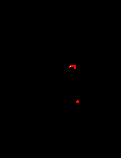
\includegraphics[width=\textwidth]{Data/results//Deeplabv3/BONBID-HIE 2023/5_1.nii_seg_err_2.png}
\end{minipage}
\begin{minipage}{0.099\textwidth}
\centering

\includegraphics[width=\textwidth]{Data/results//UMamba_2d_bot/BONBID-HIE 2023/5_1.nii_seg_err_2.png}
\end{minipage}
\begin{minipage}{0.099\textwidth}
\centering

\includegraphics[width=\textwidth]{Data/results//UMamba_3d_bot/BONBID-HIE 2023/5_1.nii_seg_err_2.png}
\end{minipage}
\end{minipage}\\%

\vspace{0.05cm}
\begin{minipage}{\textwidth}
\centering
\begin{minipage}{0.33\textwidth}
\centering
\rotatebox{90}{\tiny \textbf{Subject 6} }
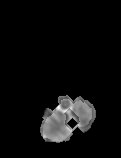
\includegraphics[width=0.3\textwidth]{Data/results//Unet/BONBID-HIE 2023/6_1.nii_src_2.png}%
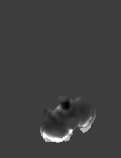
\includegraphics[width=0.3\textwidth]{Data/results//Unet/BONBID-HIE 2023/6_1.nii_src2_2.png}%
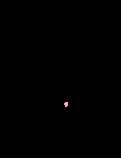
\includegraphics[width=0.3\textwidth]{Data/results//Unet/BONBID-HIE 2023/6_1.nii_gt_2.png}
\end{minipage}
\begin{minipage}{0.099\textwidth}
\centering
\includegraphics[width=\textwidth]{Data/results//Unet/BONBID-HIE 2023/6_1.nii_seg_err_2.png}
\end{minipage}
\begin{minipage}{0.099\textwidth}
\centering

\includegraphics[width=\textwidth]{Data/results//nnUNet2_2d/BONBID-HIE 2023/6_1.nii_seg_err_2.png}
\end{minipage}
\begin{minipage}{0.099\textwidth}
\centering

\includegraphics[width=\textwidth]{Data/results//nnUNet2_3d_fullres/BONBID-HIE 2023/6_1.nii_seg_err_2.png}
\end{minipage}
\begin{minipage}{0.099\textwidth}
\centering
\includegraphics[width=\textwidth]{Data/results//Deeplabv3/BONBID-HIE 2023/6_1.nii_seg_err_2.png}
\end{minipage}
\begin{minipage}{0.099\textwidth}
\centering

\includegraphics[width=\textwidth]{Data/results//UMamba_2d_bot/BONBID-HIE 2023/6_1.nii_seg_err_2.png}
\end{minipage}
\begin{minipage}{0.099\textwidth}
\centering

\includegraphics[width=\textwidth]{Data/results//UMamba_3d_bot/BONBID-HIE 2023/6_1.nii_seg_err_2.png}
\end{minipage}
\end{minipage}\\%

\vspace{0.05cm}
\begin{minipage}{\textwidth}
\centering
\begin{minipage}{0.33\textwidth}
\centering
\rotatebox{90}{\tiny \textbf{Subject 7} }
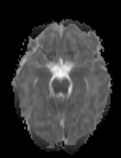
\includegraphics[width=0.3\textwidth]{Data/results//Unet/BONBID-HIE 2023/7_1.nii_src_2.png}%
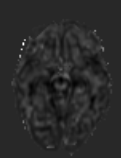
\includegraphics[width=0.3\textwidth]{Data/results//Unet/BONBID-HIE 2023/7_1.nii_src2_2.png}%
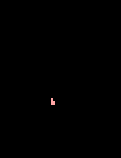
\includegraphics[width=0.3\textwidth]{Data/results//Unet/BONBID-HIE 2023/7_1.nii_gt_2.png}
\end{minipage}
\begin{minipage}{0.099\textwidth}
\centering
\includegraphics[width=\textwidth]{Data/results//Unet/BONBID-HIE 2023/7_1.nii_seg_err_2.png}
\end{minipage}
\begin{minipage}{0.099\textwidth}
\centering

\includegraphics[width=\textwidth]{Data/results//nnUNet2_2d/BONBID-HIE 2023/7_1.nii_seg_err_2.png}
\end{minipage}
\begin{minipage}{0.099\textwidth}
\centering

\includegraphics[width=\textwidth]{Data/results//nnUNet2_3d_fullres/BONBID-HIE 2023/7_1.nii_seg_err_2.png}
\end{minipage}
\begin{minipage}{0.099\textwidth}
\centering
\includegraphics[width=\textwidth]{Data/results//Deeplabv3/BONBID-HIE 2023/7_1.nii_seg_err_2.png}
\end{minipage}
\begin{minipage}{0.099\textwidth}
\centering

\includegraphics[width=\textwidth]{Data/results//UMamba_2d_bot/BONBID-HIE 2023/7_1.nii_seg_err_2.png}
\end{minipage}
\begin{minipage}{0.099\textwidth}
\centering
\includegraphics[width=\textwidth]{Data/results//UMamba_3d_bot/BONBID-HIE 2023/7_1.nii_seg_err_2.png}
\end{minipage}
\end{minipage}\\%

\vspace{0.05cm}
\begin{minipage}{\textwidth}
\centering
\begin{minipage}{0.33\textwidth}
\centering
\rotatebox{90}{\tiny \textbf{Subject 8} }
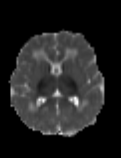
\includegraphics[width=0.3\textwidth]{Data/results//Unet/BONBID-HIE 2023/8_1.nii_src_2.png}%
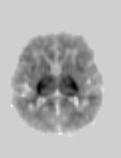
\includegraphics[width=0.3\textwidth]{Data/results//Unet/BONBID-HIE 2023/8_1.nii_src2_2.png}%

\includegraphics[width=0.3\textwidth]{Data/results//Unet/BONBID-HIE 2023/8_1.nii_gt_2.png}
\end{minipage}
\begin{minipage}{0.099\textwidth}
\centering

\includegraphics[width=\textwidth]{Data/results//Unet/BONBID-HIE 2023/8_1.nii_seg_err_2.png}
\end{minipage}
\begin{minipage}{0.099\textwidth}
\centering

\includegraphics[width=\textwidth]{Data/results//nnUNet2_2d/BONBID-HIE 2023/8_1.nii_seg_err_2.png}
\end{minipage}
\begin{minipage}{0.099\textwidth}
\centering

\includegraphics[width=\textwidth]{Data/results//nnUNet2_3d_fullres/BONBID-HIE 2023/8_1.nii_seg_err_2.png}
\end{minipage}
\begin{minipage}{0.099\textwidth}
\centering

\includegraphics[width=\textwidth]{Data/results//Deeplabv3/BONBID-HIE 2023/8_1.nii_seg_err_2.png}
\end{minipage}
\begin{minipage}{0.099\textwidth}
\centering

\includegraphics[width=\textwidth]{Data/results//UMamba_2d_bot/BONBID-HIE 2023/8_1.nii_seg_err_2.png}
\end{minipage}
\begin{minipage}{0.099\textwidth}
\centering

\includegraphics[width=\textwidth]{Data/results//UMamba_3d_bot/BONBID-HIE 2023/8_1.nii_seg_err_2.png}
\end{minipage}
\end{minipage}\\%

\vspace{0.05cm}
\begin{minipage}{\textwidth}
\centering
\begin{minipage}{0.33\textwidth}
\centering
\rotatebox{90}{\tiny \textbf{Subject 9} }
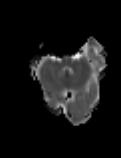
\includegraphics[width=0.3\textwidth]{Data/results//Unet/BONBID-HIE 2023/9_1.nii_src_2.png}%
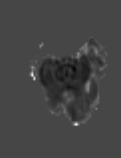
\includegraphics[width=0.3\textwidth]{Data/results//Unet/BONBID-HIE 2023/9_1.nii_src2_2.png}%
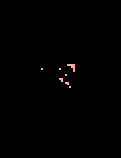
\includegraphics[width=0.3\textwidth]{Data/results//Unet/BONBID-HIE 2023/9_1.nii_gt_2.png}
\end{minipage}
\begin{minipage}{0.099\textwidth}
\centering

\includegraphics[width=\textwidth]{Data/results//Unet/BONBID-HIE 2023/9_1.nii_seg_err_2.png}
\end{minipage}
\begin{minipage}{0.099\textwidth}
\centering

\includegraphics[width=\textwidth]{Data/results//nnUNet2_2d/BONBID-HIE 2023/9_1.nii_seg_err_2.png}
\end{minipage}
\begin{minipage}{0.099\textwidth}
\centering

\includegraphics[width=\textwidth]{Data/results//nnUNet2_3d_fullres/BONBID-HIE 2023/9_1.nii_seg_err_2.png}
\end{minipage}
\begin{minipage}{0.099\textwidth}
\centering
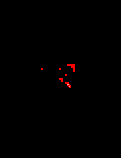
\includegraphics[width=\textwidth]{Data/results//Deeplabv3/BONBID-HIE 2023/9_1.nii_seg_err_2.png}
\end{minipage}
\begin{minipage}{0.099\textwidth}
\centering

\includegraphics[width=\textwidth]{Data/results//UMamba_2d_bot/BONBID-HIE 2023/9_1.nii_seg_err_2.png}
\end{minipage}
\begin{minipage}{0.099\textwidth}
\centering

\includegraphics[width=\textwidth]{Data/results//UMamba_3d_bot/BONBID-HIE 2023/9_1.nii_seg_err_2.png}
\end{minipage}
\end{minipage}\\%

\vspace{0.05cm}

\caption{Visual comparison of slices of images, ground truth and segmentations created by models for BONBID-HIE 2023 segmentations. Incorrectly classified pixels are dark red. Legend for subjects is in table \ref{tab:bonbidtestlegend}.}
\label{fig:bonbidslicecomparison}
\end{figure}

\begin{table}
\centering
\begin{tabular}{l c c}
\hline
\textbf{Subject} & \textbf{Number of regions} & \textbf{Brain volume percentage} \\
\hline
1 & 0   & 0 \% \\
2 & 14  & 0{,}98 \% \\
3 & 27  & 8{,}32 \% \\
4 & 2   & 0{,}06 \% \\
5 & 2   & 0{,}035 \% \\
6 & 20  & 0{,}44 \% \\
7 & 1   & 0{,}037 \% \\
8 & 3   & 59{,}31 \% \\
9 & 117 & 1{,}44 \% \\
\hline
\end{tabular}
\caption{Overview of number of regions and brain volume percentage for test subjects of BONBID-HIE 2023 dataset.}
\label{tab:bonbidtestlegend}
\end{table}

\begin{figure}
\centering
\input{Data/results/tacr_aseg_img_2.tex}
\caption{Visual comparison of slices of images, ground truth and segmentations created by models for TAČR 6-HIE (aseg) segmentations. Incorrectly classified pixels are dark red.}
\label{fig:tacrasegslicecomparison}
\end{figure}

\begin{figure}
\centering
\caption{Visual comparison of slices of images, ground truth and segmentations created by models for TAČR 6-HIE (aseg+aparc) segmentations. Incorrectly classified pixels are dark red}
\label{fig:tacraparcslicecomparison}
\begin{minipage}{\textwidth}
\centering
\begin{minipage}{0.33\textwidth}
\hfill
\begin{minipage}{0.3\textwidth}
\rotatebox{90}{Image}
\end{minipage}
\begin{minipage}{0.3\textwidth}
\rotatebox{90}{Ground truth}
\end{minipage}
\hfill
\end{minipage}
\begin{minipage}{0.099\textwidth}
\centering
\rotatebox{90}{U-net (3D)}
\end{minipage}
\begin{minipage}{0.099\textwidth}
\centering
\rotatebox{90}{nnUNet (2D)}
\end{minipage}
\begin{minipage}{0.099\textwidth}
\centering
\rotatebox{90}{nnUNet (3D)}
\end{minipage}
\begin{minipage}{0.099\textwidth}
\centering
\rotatebox{90}{DeepLab (v3)}
\end{minipage}
\begin{minipage}{0.099\textwidth}
\centering
\rotatebox{90}{U-Mamba (2D bot)}
\end{minipage}
\begin{minipage}{0.099\textwidth}
\centering
\rotatebox{90}{U-Mamba (3D bot)}
\end{minipage}
\end{minipage}
\begin{minipage}{\textwidth}
\centering
\begin{minipage}{0.33\textwidth}
\centering
\rotatebox{90}{\tiny \textbf{Subject 15} }
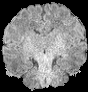
\includegraphics[width=0.3\textwidth]{Data/results//Unet/TACR 6-HIE aseg+aparc/15_1.nii_src_2.png}%
%\includegraphics[width=0.3\textwidth]{Data/results//Unet/TACR 6-HIE aseg+aparc/15_1.nii_src2_2.png}%

\includegraphics[width=0.3\textwidth]{Data/results//Unet/TACR 6-HIE aseg+aparc/15_1.nii_gt_2.png}
\end{minipage}
\begin{minipage}{0.099\textwidth}
\centering

\includegraphics[width=\textwidth]{Data/results//Unet/TACR 6-HIE aseg+aparc/15_1.nii_seg_err_2.png}
\end{minipage}
\begin{minipage}{0.099\textwidth}
\centering

\includegraphics[width=\textwidth]{Data/results//nnUNet2_2d/TACR 6-HIE aseg+aparc/15_1.nii_seg_err_2.png}
\end{minipage}
\begin{minipage}{0.099\textwidth}
\centering

\includegraphics[width=\textwidth]{Data/results//nnUNet2_3d_fullres/TACR 6-HIE aseg+aparc/15_1.nii_seg_err_2.png}
\end{minipage}
\begin{minipage}{0.099\textwidth}
\centering

\includegraphics[width=\textwidth]{Data/results//Deeplabv3/TACR 6-HIE aseg+aparc/15_1.nii_seg_err_2.png}
\end{minipage}
\begin{minipage}{0.099\textwidth}
\centering

\includegraphics[width=\textwidth]{Data/results//UMamba_2d_bot/TACR 6-HIE aseg+aparc/15_1.nii_seg_err_2.png}
\end{minipage}
\begin{minipage}{0.099\textwidth}
\centering

\includegraphics[width=\textwidth]{Data/results//UMamba_3d_bot/TACR 6-HIE aseg+aparc/15_1.nii_seg_err_2.png}
\end{minipage}
\end{minipage}\\%

\vspace{0.05cm}
\begin{minipage}{\textwidth}
\centering
\begin{minipage}{0.33\textwidth}
\centering
\rotatebox{90}{\tiny \textbf{Subject 8} }

\includegraphics[width=0.3\textwidth]{Data/results//Unet/TACR 6-HIE aseg+aparc/8_1.nii_src_2.png}%
%
\includegraphics[width=0.3\textwidth]{Data/results//Unet/TACR 6-HIE aseg+aparc/8_1.nii_src2_2.png}%

\includegraphics[width=0.3\textwidth]{Data/results//Unet/TACR 6-HIE aseg+aparc/8_1.nii_gt_2.png}
\end{minipage}
\begin{minipage}{0.099\textwidth}
\centering

\includegraphics[width=\textwidth]{Data/results//Unet/TACR 6-HIE aseg+aparc/8_1.nii_seg_err_2.png}
\end{minipage}
\begin{minipage}{0.099\textwidth}
\centering

\includegraphics[width=\textwidth]{Data/results//nnUNet2_2d/TACR 6-HIE aseg+aparc/8_1.nii_seg_err_2.png}
\end{minipage}
\begin{minipage}{0.099\textwidth}
\centering

\includegraphics[width=\textwidth]{Data/results//nnUNet2_3d_fullres/TACR 6-HIE aseg+aparc/8_1.nii_seg_err_2.png}
\end{minipage}
\begin{minipage}{0.099\textwidth}
\centering

\includegraphics[width=\textwidth]{Data/results//Deeplabv3/TACR 6-HIE aseg+aparc/8_1.nii_seg_err_2.png}
\end{minipage}
\begin{minipage}{0.099\textwidth}
\centering

\includegraphics[width=\textwidth]{Data/results//UMamba_2d_bot/TACR 6-HIE aseg+aparc/8_1.nii_seg_err_2.png}
\end{minipage}
\begin{minipage}{0.099\textwidth}
\centering

\includegraphics[width=\textwidth]{Data/results//UMamba_3d_bot/TACR 6-HIE aseg+aparc/8_1.nii_seg_err_2.png}
\end{minipage}
\end{minipage}\\%

\vspace{0.05cm}

\end{figure}

\section{Conclusion}
We implemented and utilized existing neural networks for four segmentation tasks. As the results show our implementations and configurations have not achieved satisfactory results for the BONBID-HIE 2023 dataset, where on selected data split we achieved maximum median DICE of only around 0.4. 

Our implementation of U-net with 3D convolutions achieved worst score of approximately 0.83 in iSeg 2019 segmentation task. On the other hand, similar network architecture configured by nnUnet  achieved best DICE score (around 0.92). In both segmentation tasks of TAČR 6 - HIE dataset our implementation achieved the best scores (around 10\% better than nnUnet). This result is quite surprising, as we were not expecting to surpass nnUnet with such a simple architecture without extended fine tuning.

Overall the results are not satisfactory for clinical application and further research is needed. One limitation in our methodology which should be addressed is the lack of cross validation, which would provide more robust evaluation of models in the case of such small datasets, which were examined.


%\subsection{A Subsection Sample}
%Please note that the first paragraph of a section or subsection is
%not indented. The first paragraph that follows a table, figure,
%equation etc. does not need an indent, either.

%Subsequent paragraphs, however, are indented.

%\subsubsection{Sample Heading (Third Level)} Only two levels of
%headings should be numbered. Lower level headings remain unnumbered;
%they are formatted as run-in headings.

%\paragraph{Sample Heading (Fourth Level)}
%The contribution should contain no more than four levels of
%headings. Table~\ref{tab1} gives a summary of all heading levels.

%\begin{table}
%\caption{Table captions should be placed above the
%tables.}\label{tab1}
%\begin{tabular}{|l|l|l|}
%\hline
%Heading level &  Example & Font size and style\\
%\hline
%Title (centered) &  {\Large\bfseries Lecture Notes} & 14 point, bold\\
%1st-level heading &  {\large\bfseries 1 Introduction} & 12 point, bold\\
%2nd-level heading & {\bfseries 2.1 Printing Area} & 10 point, bold\\
%3rd-level heading & {\bfseries Run-in Heading in Bold.} Text follows & 10 point, bold\\
%4th-level heading & {\itshape Lowest Level Heading.} Text follows & 10 point, italic\\
%\hline
%\end{tabular}
%\end{table}


%\noindent Displayed equations are centered and set on a separate
%line.
%\begin{equation}
%x + y = z
%\end{equation}
%Please try to avoid rasterized images for line-art diagrams and
%schemas. Whenever possible, use vector graphics instead (see
%Fig.~\ref{fig1}).

%\begin{figure}
%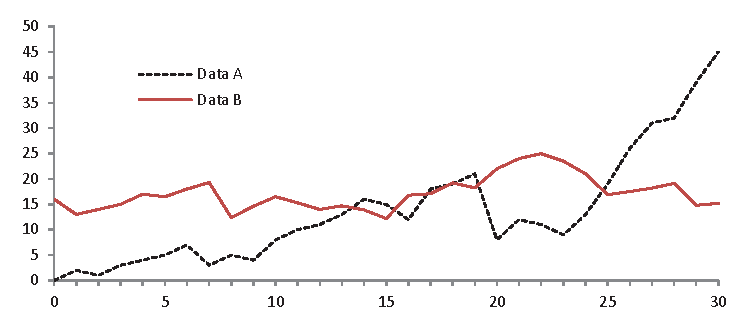
\includegraphics[width=\textwidth]{fig1.eps}
%\caption{A figure caption is always placed below the illustration.
%Please note that short captions are centered, while long ones are
%justified by the macro package automatically.} %\label{fig1}
%\end{figure}

%\begin{theorem}
%This is a sample theorem. The run-in heading is set in bold, while
%the following text appears in italics. Definitions, lemmas,
%propositions, and corollaries are styled the same way.
%\end{theorem}
%
% the environments 'definition', 'lemma', 'proposition', 'corollary',
% 'remark', and 'example' are defined in the LLNCS documentclass as well.
%
%\begin{proof}
%Proofs, examples, and remarks have the initial word in italics,
%while the following text appears in normal font.
%\end{proof}
%For citations of references, we prefer the use of square brackets
%and consecutive numbers. Citations using labels or the author/year
%convention are also acceptable. The following bibliography provides
%a sample reference list with entries for journal
%articles~\cite{ref_article1}, an LNCS chapter~\cite{ref_lncs1}, a
%book~\cite{ref_book1}, proceedings without editors~\cite{ref_proc1},
%and a homepage~\cite{ref_url1}. Multiple citations are grouped
%\cite{ref_article1,ref_lncs1,ref_book1},
%\cite{ref_article1,ref_book1,ref_proc1,ref_url1}.

\begin{credits}
\subsubsection{\ackname}This article was supported by Grant No. SP2025/016 Parallel processing of Big Data XII, VSB Technical University of Ostrava, Czech Republic.

\end{credits}
%
% ---- Bibliography ----
%
% BibTeX users should specify bibliography style 'splncs04'.
% References will then be sorted and formatted in the correct style.
%
\bibliographystyle{splncs04}
\bibliography{bibliography}
%
%\begin{thebibliography}{8}
%\bibitem{ref_article1}
%Author, F.: Article title. Journal \textbf{2}(5), 99--110 (2016)

%\bibitem{ref_lncs1}
%Author, F., Author, S.: Title of a proceedings paper. In: Editor,
%F., Editor, S. (eds.) CONFERENCE 2016, LNCS, vol. 9999, pp. 1--13.
%Springer, Heidelberg (2016). \doi{10.10007/1234567890}

%\bibitem{ref_book1}
%Author, F., Author, S., Author, T.: Book title. 2nd edn. Publisher,
%Location (1999)

%\bibitem{ref_proc1}
%Author, A.-B.: Contribution title. In: 9th International Proceedings
%on Proceedings, pp. 1--2. Publisher, Location (2010)

%\bibitem{ref_url1}
%LNCS Homepage, \url{http://www.springer.com/lncs}, last accessed 2023/10/25
%\end{thebibliography}
\end{document}
